In this section, the results of the model applied to the environment are illustrated. The first sub-section shows an evaluation of the model based on the metrics stated in \nameref{sub:Metrics}. The last sub-section shows a Justification of the model, which is a comparison of its performance against the \nameref{sub:Benchmark}.
%%%%%%%%%%%%%%%%%%%%%%%%%%%%%%%%%%%%%%%%%%%%
\subsection{Model Evaluation and Validation}
%%%%%%%%%%%%%%%%%%%%%%%%%%%%%%%%%%%%%%%%%%%%
% The final model’s qualities — such as parameters — are evaluated in detail. Some type of analysis is used to validate the robustness of the model’s solution.
The reason to implement a custom reward (CR) + skipped frames (SF) system as explained in \nameref{sub:Refinement}  was to favor the creation of momentum. Momentum is the key physical attribute to solve this environment which at the same time is proportional to the speed of the car and its mass. However, since we do not have control over its mass, the only variable to favor in the environment is velocity, that is why all CR + SF focus on increasing the speed of the car. The results compared to a normal environment reward (ER) after the implementation of the DQN are shown in Table\ref{tab:CR+SF}.
\begin{table}[h]
\centering
\begin{tabular}{|c|c|c|c|}
\hline
                                                                                             & \textbf{\begin{tabular}[c]{@{}c@{}}Environment's\\ Reward (ER)\end{tabular}} & \textbf{\begin{tabular}[c]{@{}c@{}}ER+Custom\\ Reward (CR)\end{tabular}} & \textbf{\begin{tabular}[c]{@{}c@{}}CR+Skipped\\ Frames (SF)\end{tabular}} \\ \hline
\textbf{\begin{tabular}[c]{@{}c@{}}Episodes required to\\ find a solution\end{tabular}}      & \textgreater 2000                                                            & \textgreater 400                                                         & \textgreater 200                                                     \\ \hline
\textbf{\begin{tabular}[c]{@{}c@{}}Best 100 average \\ Reward in 2000 episodes\end{tabular}} & $<$ -190                                                                          & -160 to -150                                                               & -130 to -120                                                           \\ \hline
\end{tabular}
\caption{ER vs CR+SF}
\label{tab:CR+SF}
\end{table}

.

%%%%%%%%%%%%%%%%%%%%%%%%%%
\subsection{Justification}
%%%%%%%%%%%%%%%%%%%%%%%%%%
% The final results are compared to the benchmark result or threshold with some type of statistical analysis. Justification is made as to whether the final model and solution is significant enough to have adequately solved the problem.

The results of the model against the benchmarks stated for this projects are presented in Table\ref{tab:modelVSbenchmarks}

\begin{table}[h]
\centering
\begin{tabular}{|c|c|c|c|c|}
\hline
                                                                                                   & \textbf{\begin{tabular}[c]{@{}c@{}}Random\\ algorithm\end{tabular}} & \textbf{\begin{tabular}[c]{@{}c@{}}First in Leader\\ Board (jing582)\end{tabular}} & \textbf{\begin{tabular}[c]{@{}c@{}}Second in Leader\\ Board \\ (DaveLeong)\end{tabular}} & \textbf{DQN Model} \\ \hline
\textbf{\begin{tabular}[c]{@{}c@{}}Episodes required \\ to converge \\ to a solution\end{tabular}} & \begin{tabular}[c]{@{}c@{}}No solution\\ Found\end{tabular}         & 1119                                                                               & 1967                                                                                     & $<$1000               \\ \hline
\textbf{\begin{tabular}[c]{@{}c@{}}100 average \\ range in Testing \\ the algorithm\end{tabular}}  & -200                                                                & \textgreater  -110                                                                  & \textgreater  -110                                                                        & -130 to -120       \\ \hline
\end{tabular}
\caption{Deep Q learning model against Benchmarks}
\label{tab:modelVSbenchmarks}
\end{table}
As it can be seen in the table above, our model is much better than a random algorithm where the 100 average in testing is -200, whereas the DQN model result is between -130 and -120. On the other hand, both leaders got better 100 average results than the DQN model. However, the speed of convergence of the DQN was faster, since it required less than 1000 episodes to converge to a solution. Overall we can state that the DQN is a good candidate to solve the Mountain Car problem, and to strengthen the statement we could find the graph of the learning process of the model in Figure\ref{fig:Learning}

\begin{figure}[h]
\centering
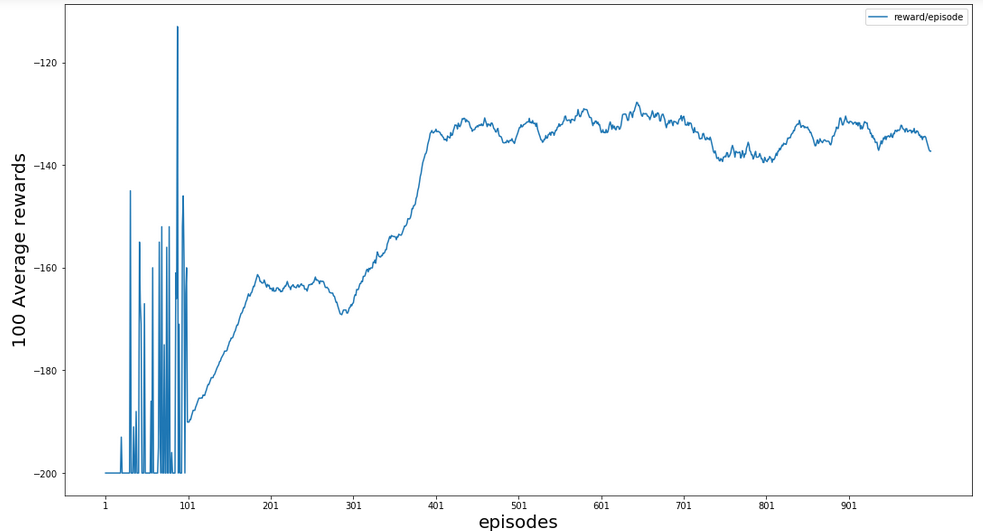
\includegraphics[width=0.8\textwidth]{LearningProcessDQN.png}
\caption{Learning process of the Deep Q learning approach to the Mountain Car problem}
\label{fig:Learning} 
\end{figure}

.
